\documentclass[12pt,aspectratio=169]{beamer}
\usetheme[version=2024]{iiasa}

\AtBeginSection{}

\title{MESSAGEix-Transport/-GLOBIOM}
\subtitle{Participant model in the EDITS Model Complementarity Exercise (MCE)}
\institute{
  Energy, Climate, and Environment (ECE) Program \\
  International Institute for Applied Systems Analysis (IIASA)}

\date{
  \texorpdfstring{EDITS Annual Meeting BOG 10.1 — Thursday, 10 October 2024}%
  {2024-10-10}}

\author{\texorpdfstring{Paul Kishimoto, Aneeque Javaid, Takuya Hara, Volker~Krey, Bas van Ruijven\\
  \href{mailto:kishimot@iiasa.ac.at}{\ttfamily \scriptsize <kishimot@iiasa.ac.at>}%
  }{Paul Natsuo Kishimoto <kishimot@iiasa.ac.at>}}

\usepackage[
  maxnames = 1,
  style = authoryear,
  giveninits,
  terseinits,
  maxcitenames = 3,
  ]{biblatex}
\addbibresource{all.bib}

\usepackage{minted}

\begin{document}

\maketitle

\begin{frame}
\frametitle{MESSAGEix-Transport}
\framesubtitle{A very brief introduction}

\tableofcontents

\end{frame}

\section{MESSAGEix-Transport}
\subsection{Model code \& data}

\begin{frame}
\frametitle{Model code \& data}

MESSAGEix-Transport code and data are included and developed as part of \texttt{message-ix-models}:

\bigskip
{\Large
Documentation: \href{https://docs.messageix.org/models}{docs.messageix.org/models}

\smallskip
Code \& data: \href{https://github.com/iiasa/message-ix-models}{github.com/iiasa/message-ix-models}

\medskip
\href{https://github.com/search?q=repo\%3Aiiasa\%2Fmessage-ix-models+label\%3Atransport\&type=issues}{Issues and pull requests} ← follow along or join development
}

\end{frame}

\subsection{About the model: purpose, requirements, structure}

\begin{frame}[allowframebreaks]
\frametitle{MESSAGEix-GLOBIOM model family}
Linear optimization (LP)-based \structure{integrated assessment models (IAMs)}:
\begin{itemize}
  \item ‘Integrative’ of the full global energy-economic system.
  \item For ‘assessment’ of future scenarios (incl. climate policy)\\and their effects on \structure{global total emissions}.
  \item Linked to MACRO (CGE) \& GLOBIOM (land use, via emulator) models.
  \item Spatial resolution: 12 regions.
  \item Temporal scope \& resolution: 5- and 10-year periods to 2110.
\end{itemize}

\medskip
A \structure{‘family’} because:
\begin{itemize}
  \item Many model \structure{variants} with similar but different structure: spatial scope (single countries)/resolution (<> 12 regions); technologies; constraints.
  \item e.g. MESSAGEix-Nexus, MESSAGEix-Materials, MESSAGEix-Buildings.
\end{itemize}

\framebreak
\href{https://github.com/iiasa/message-ix-models}{\ttfamily message-ix-models} —a Python package for code to \structure{build} (set up structure + add data) → \structure{solve} → \structure{report} (postprocess) MESSAGEix-GLOBIOM scenarios.
\begin{itemize}
  \item Free and open source since 2021.
  \item 14,000+ lines of Python code; submodules for model variants.
  \item Documentation, changelog, test suite, automated quality control (QC)\\and validation.
  \item Not \emph{all} MESSAGEix-GLOBIOM applications and code (some still private),\\but a growing share.
  \item >1 ‘snapshot’ of the base/global MESSAGEix-GLOBIOM available on Zenodo (\href{https://docs.messageix.org/projects/models/en/latest/api/model-snapshot.html}{docs}).
\end{itemize}

\end{frame}

\begin{frame}
\frametitle{MESSAGEix-Transport: a variant in the family}

MESSAGEix-GLOBIOM transport structure is \structure{aggregated/low resolution}.
\begin{itemize}
  \item Technologies like \texttt{t=elec\_trp}: sum total of all transport modes, vehicle types, powertrains that input commodity \texttt{c=electr}.
  \item Input in [GW·a] of (final) energy; output in [GW·a] of ‘useful energy’.
  \item Exogenous%
  \footnote{Aggregate price elasticity via MACRO.}
  \texttt{demand} projection for this useful energy.
\end{itemize}

MESSAGEix-Transport structure is \structure{\emph{slightly} higher resolution}.
\begin{itemize}
  \item Transport \texttt{demand} expressed in PDT [km] or freight volume [t·km], projected using outside calculation, data sources, and models.
  \item Intermediate VDT [km] for 5 passenger and 2 freight modes.
  \item 1–10 technologies for each (service, mode) → distinct costs, efficiencies, constraints. \texttt{CAP}-acity variable measures vehicle stock [10⁶]; \texttt{ACT}-ivity measures VDT [10⁹ km/a].
\end{itemize}
\end{frame}

\begin{frame}
\frametitle{Data stages}
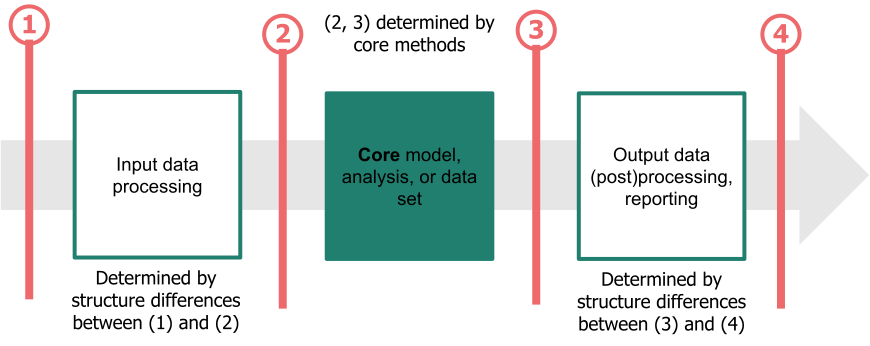
\includegraphics[width=\columnwidth]{data-stages}
\end{frame}

\begin{frame}
\frametitle{Purpose and applications}

These are most importantly \structure{varied}—this is a tool meant to be used for multiple purposes—but include:
\begin{itemize}
  \item Add transport sector detail to scenarios \& reported/output data while \structure{retaining MESSAGEix-GLOBIOM's scope and detail} in representation of energy supply, land use, other sectors.
  \item Provide \structure{aggregate outputs to calibrate} the ‘base’ representation

  (with \texttt{t=elec\_trp} technologies).%
  \footnote{e.g. for the ScenarioMIP / SSP (2024) process.}
  \item \structure{Enable connections to transport literature and data}:
  \begin{itemize}
    \item Input data from higher-resolution (if not “bottom-up”) models.

    e.g. ITF-OECD ‘PASTA’ in the EDITS MCE.
    \item Calibrate using data on activity; mode share; vehicle stocks/sales; techno-economic attributes; etc. common in transport research domain.
  \end{itemize}
\end{itemize}
\end{frame}

\subsection{Development and calibration; \texttt{genno}}
\begin{frame}
\frametitle{Development and calibration}

\begin{itemize}
  \item Initial structure from \textcite{mccollum-2017} + extensive data updates.
  \item New system for \structure{build} and \structure{report} modeling steps.
  \item Workflow automation and testing.
\end{itemize}

\medskip
These serve some \structure{process and usability goals}:
\begin{enumerate}
  \item Provide \structure{flexibility} for the varied applications (above),
  \item Enable \structure{repeatable, reproducible} workflows.
  \begin{itemize}
    \item Push-button to rebuild the model from scratch w/ updated data.
    \item Automated ‘nightly’ runs.
  \end{itemize}
  \item Reduce development/maintenance burden and facilitate collaboration.

  (Only <2 FTE working on this implementation.)
\end{enumerate}
\end{frame}

\begin{frame}[allowframebreaks,fragile]
\frametitle{Implementation detail: input data workflows}

MESSAGEix-Transport calibration and input data workflows are \structure{composed} using \structure{small functions}/steps: e.g. below \verb@logit@, \verb@mul@, \verb@factor_pdt@.
\begin{minted}{python}
# Mode shares
c.add(ms, "logit", cost, sw, "lambda:", y), dict(dim="t")
# Total PDT (n, t, y), with modes for the 't' dimension
c.add(pdt_nyt + "0", "mul", pdt_ny, ms)
# Scenario-specific adjustment factors
c.add("pdt factor:n-y-t", "factor_pdt", n, y, t_modes, "config")
\end{minted}

\medskip
Because small, these are \structure{reusable}, \structure{testable}, easy to document/read (\structure{transparent}), etc.

\framebreak
\begin{columns}
\column[T]{0.6\paperwidth}
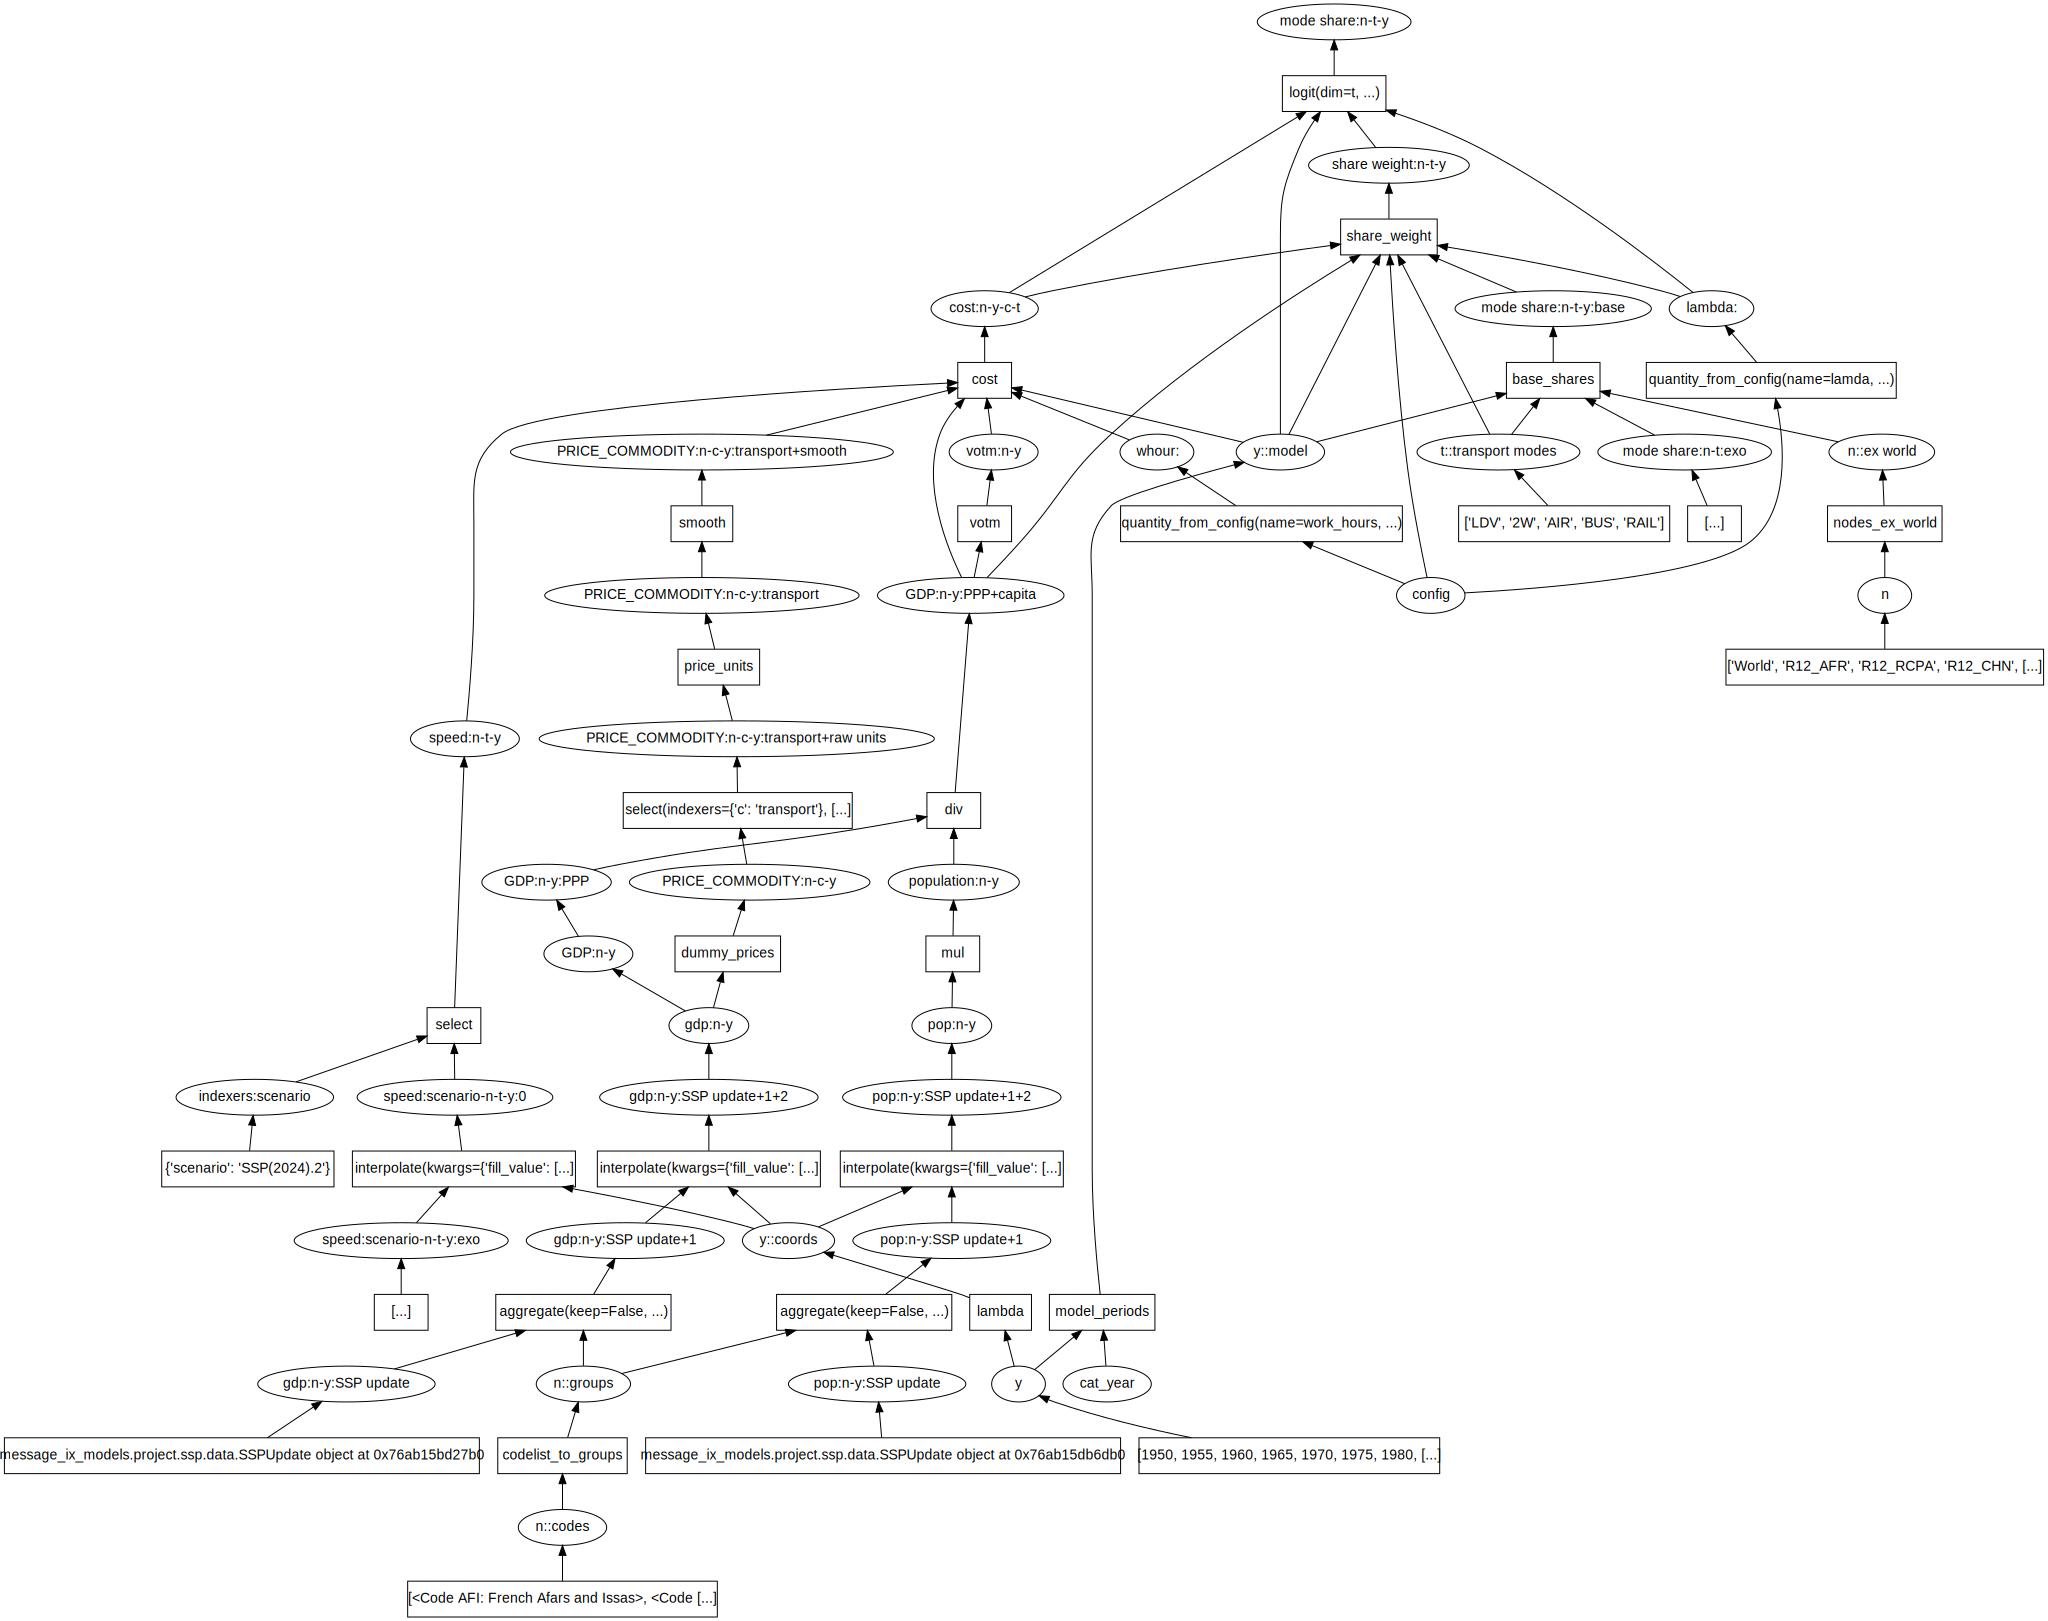
\includegraphics[width=\columnwidth]{transport-build-debug.pdf}
\column[T]{0.35\paperwidth}
Available data requires to set up \& manipulate complicated chains of these atomic steps.

\medskip
Well-structured calculations make it easier to:
\begin{itemize}
  \item Separate assumptions/ settings/data from methods.
  \item Make steps ‘agnostic’ to e.g. spatio-temporal resolution.
  \item “Prune-and-graft” to swap methods or data sources.
\end{itemize}
\end{columns}
\end{frame}

\subsection{Ongoing work \& future directions}

\begin{frame}
\frametitle{Ongoing work \& future directions}

\begin{enumerate}
  \item \href{https://iiasa.ac.at/projects/edits}{EDITS} Model Complementarity Exercise (MCE):

  \structure{Prune} default activity projection (modified \textcite{schafer-2009} method)…

  \structure{…graft} on data from ITF-OECD PASTA with appropriate transformations.
  \item Direct integration with MESSAGEix-Materials.
  \begin{itemize}
    \item Growth of vehicle \texttt{CAP} → inflows of materials used in vehicles.
    \item Growth of mode \texttt{ACT} → inflows of materials used in infrastructures.
  \end{itemize}
  \item Trip-based activity projection

  at higher resolution → aggregated to core units of analysis.
  \item Similar links to other models with higher resolution but narrower scope:
  \begin{itemize}
    \item Water freight.
    \item Air passenger \& freight.
  \end{itemize}
\end{enumerate}

\end{frame}

\section{Application in the EDITS MCE}

\begin{frame}[allowframebreaks]
\frametitle{Application in the EDITS MCE}

MCE research question (not yet set…) turns on \structure{shared mobility}.
\begin{itemize}
  \item A broad basket of concepts and phenomena.
  \item In particular: effects of low vs. high amounts of sharing of passenger LDVs.
\end{itemize}

\bigskip
In MESSAGEix-Transport \structure{core representation}:

\smallskip
\texttt{demand} for LDV passenger-distance traveled (PDT) [km] is represented with dimensions (node, time period, consumer group).
\begin{itemize}
  \item \structure{\textbf{NO}} distinction between demand for “PDT in shared LDVs” vs. “PDT in non-shared LDVs” → differences across MCE scenarios not captured in the model core.
\end{itemize}

\framebreak
LDV PDT \texttt{demand} is \emph{indirectly} satisfied by one of ~8 technologies that input different energy commodities.
These…
\begin{itemize}
  \item …\texttt{output} vehicle distance traveled (VDT) [km]
  \begin{itemize}
    \item This is then transformed to PDT using a ‘pseudo-technology’ like \texttt{PHEV usage by [group]}.
    \item The ratio of \texttt{output}/\texttt{input} for this technology is parametrized using data on \structure{occupancy of LDVs}.
  \end{itemize}
  \item …have a \texttt{capacity\_factor} (\texttt{ACT}/\texttt{CAP}) in units of [km / vehicle / year].
  \begin{itemize}
    \item This is parametrized using data on \structure{vehicle utilisation}.
    \item This representation exists to report (and calibrate) \texttt{CAP} as \structure{vehicle stock}.
  \end{itemize}
\end{itemize}
\end{frame}

\begin{frame}
\frametitle{Implementation in (1→2) and (3→4)}
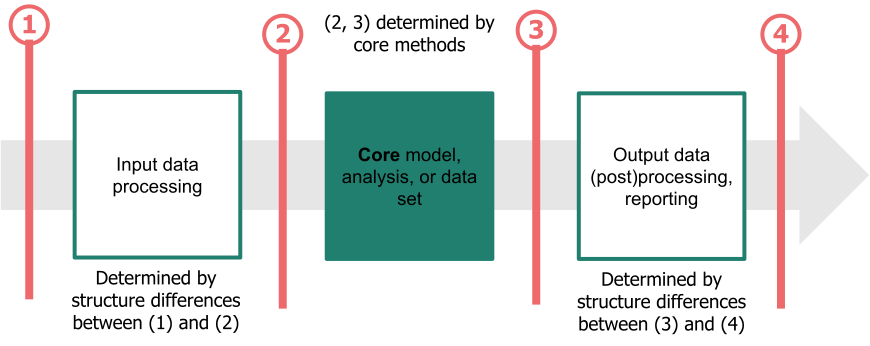
\includegraphics[width=\columnwidth]{data-stages}
\end{frame}

\begin{frame}
\frametitle{Application in the EDITS MCE III}

Methods for achieving ‘complementarity’ are chosen to balance ‘realism’ and the effort required to modify the model build — core/solve — report stages.

\medskip
\begin{enumerate}
  \item Receive PASTA data.
  \item \structure{Transform} to interoperable, standard data structure / format.
  \item \structure{Aggregate/adjust} to MESSAGEix-Transport spatio-temporal resolution.
  \item \structure{Extend or construct} time series to MESSAGEix-Transport temporal scope.
  \item \structure{Compute} input quantities (occupancy, vehicle utilisation).
  \item \structure{Broadcast} to all MESSAGEix-Transport technologies and consumer groups.
  \item \structure{Replace} (“prune and graft”) default values for parameters (5) and \texttt{demand}.
\end{enumerate}

\medskip
(2–7) done with the affordances of the flexible model implementation.
\end{frame}

\makefinalslide

\appendix

\begin{frame}[allowframebreaks]
\frametitle{References}

\printbibliography[heading=none]

\end{frame}

\end{document}
